\documentclass{../lab_class}

\usepackage{fancyhdr}
\pagestyle{fancy}
\rhead{П.\,Ю. Смирнов, 687 гр.}
\lhead{Лабораторная работа № 4.4.1, МФТИ, весна 2018}

\newcommand{\angstrom}{\text{\normalfont\AA}}

\begin{document}

%	thnx Плюсинину Павлу за данные
%	и спасибо гониометру за 1,5 пары настройки
%	и, соотв., негодные результаты своих измерений

{\Large 4.4.1 -- Амплитудная дифракционная решётка.}

\paragraph{Цель работы.}
Знакомство с работой и настройкой гониометра, определение спектральных характеристик амплитудной решётки.

В работе используются: гониометр, дифракционная решётка, ртутная лампа.

\paragraph{Теоретическая часть.}
Спектральный анализ (разложение электромагнитного излучения на монохроматические составляющие) может многое сказать о природе источника излучения. Принципиальная схема установки для изучения спектра показана на рисунке \ref{fig:scheme}: коллиматор формирует параллельный пучок света от источника, ДЭ осуществляет пространственное спектральное разложение пучка. 

\begin{figure}[H]
	\centering
	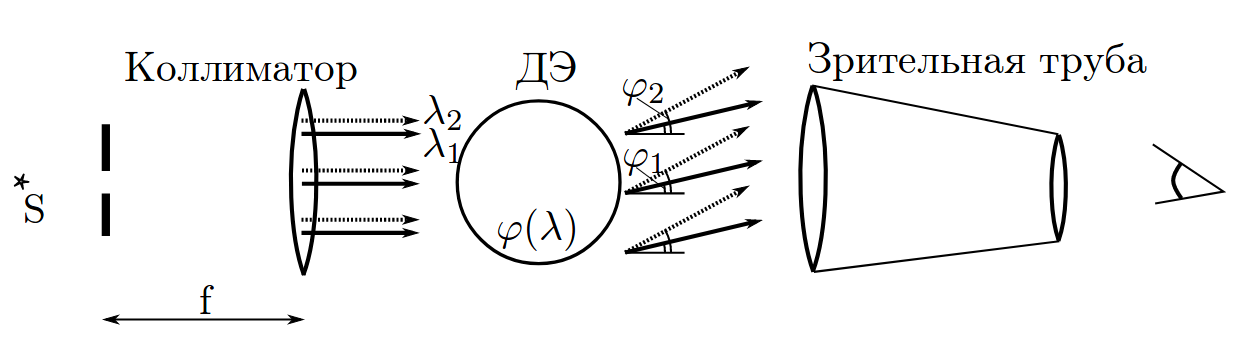
\includegraphics[width=12cm]{scheme.png}
	\caption{Схема прибора: источник-коллиматор, диспергирующий элемент, зрительная труба.}
	\label{fig:scheme}
\end{figure}

\begin{wrapfigure}{r}{0.3\textwidth}
  \vspace{-20pt}
  \begin{center}
    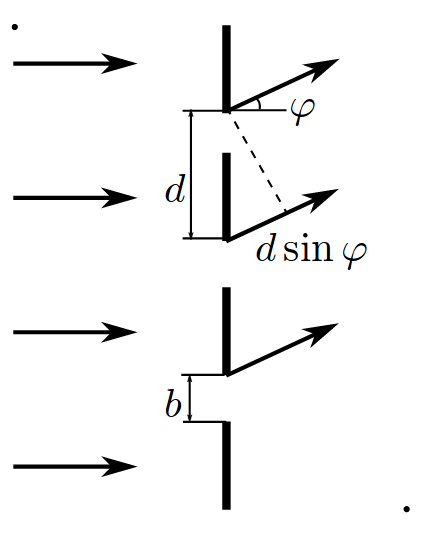
\includegraphics[width=0.28\textwidth]{lattice.png}
  \end{center}
  \vspace{-20pt}
  \caption{Дифракция световой волны на амплитудной решётке}
  \label{fig:lattice}
  \vspace{-10pt}
\end{wrapfigure}


В нашем эксперименте диспергирующим элементом является амплитудная дифракционная решетка (рис. \ref{fig:lattice}). Каждая щель становится, по принципу Гюйгенса-Френеля, источником вторичных сферических волн, интерферирующих между собой; ясно, что максимум интенсивности света на экране наблюдается только в том случае, если дифрагирующие волны приходят в одной фазе:
\begin{equation}\label{eq:main}
	d \sin \varphi = m \lambda,
\end{equation}
где $d$ -- период решетки, $\lambda$ -- длина волны, $m$ -- целое число. Коль скоро пучок света представляет собой суперпозицию монохроматических волн с длинами волн $\lambda_i$, мы наблюдаем пространственное разделение максимумов в зависимости от длины волны (соотв. цвета).

\paragraph{Эксперимент.}
В данной работе будем исследовать спектр ртути (источник -- ртутная лампа). Первым делом измерим угловые координаты (о гониометре говорить не будем) спектров ртути:

\bigskip
\begin{tabular}{|c|c|c|c|}
\hline
$\text{цвет}$ & $\varphi$ & $\sin (\varphi - \varphi_0)$ & $\lambda, \sn \m$ \\
\hline
фиолетовый	&	$13^{\circ}02^{\prime}01^{\prime \prime}$	& 0.225	&	404.7	\\ \hline
синий	&	$13^{\circ}59^{\prime}37^{\prime \prime}$	&	0.242	&	435.8	\\ \hline
голубой	&	$14^{\circ}27^{\prime}08^{\prime \prime}$	&	0.249	&	491.6	\\ \hline
зеленый	&	$15^{\circ}43^{\prime}20^{\prime \prime}$	&	0.271	&	546.1	\\ \hline
желтый	&	$16^{\circ}38^{\prime}29^{\prime \prime}$	&	0.286	&	577.0	\\ \hline
желтый	&	$16^{\circ}42^{\prime}36^{\prime \prime}$	&	0.287	&	579.1	\\ \hline
\end{tabular}
\bigskip

\pagebreak

\begin{figure}[H]
	\centering
	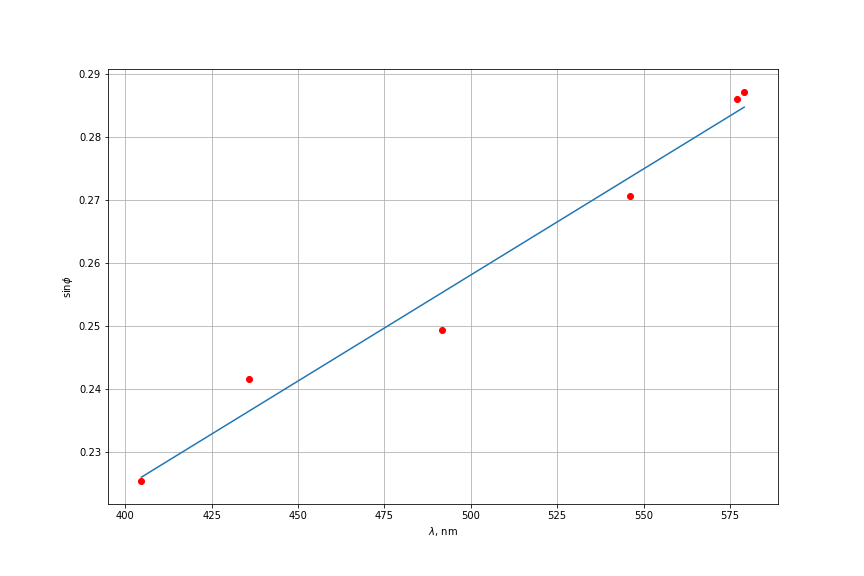
\includegraphics[width=17cm]{fig1.png}
	\caption{Зависимость пространственного спектрального разложения от длины волны.}
	\label{fig:results}
\end{figure}

Измерения ясно показывают справедливость формулы \eqref{eq:main}. По графику зависимости определим шаг решетки:

\begin{gather*}
\boxed{
	d \simeq 2890 \pm 190 \ \sn \m
	}
\end{gather*}

Заметим, что на установке $N = 500 \ \text{штрихов} / \sm \m \then d = 2000 \ \sn \m$, что мы почти и получили.

Теперь исследуем угловую дисперсию по линия жёлтого дублета в спектрах разного порядка $m$:

\begin{equation}
	D(\lambda) = \dv{\varphi}{\lambda} = \frac{m}{\sqrt{d^2 - m^2 \lambda^2}}.
\end{equation}

\bigskip
\begin{tabular}{|c|c|c|c|c|c|}
\hline
$m$ & $\text{1-ая линия}$ & $\text{2-ая линия}$ & $\Delta \varphi, \text{сек}$ & $D_{\text{exp}}$ & $D_{\text{theor}}$ \\
\hline
1	&	$16^{\circ}38^{\prime}29^{\prime \prime}$	&	$16^{\circ}42^{\prime}36^{\prime \prime}$	&	$247$	&	$11.76$	&	$16.96$	\\ \hline
-1	&	$6^{\circ}58^{\prime}00^{\prime \prime}$	&	$6^{\circ}53^{\prime}43^{\prime \prime}$	&	$-257$	&	-$12.23$	&	$-16.96$	\\ \hline
-2	&	$26^{\circ}31^{\prime}01^{\prime \prime}$	&	$26^{\circ}44^{\prime}45^{\prime \prime}$	&	$824$	&	$-39.23$	&	$-44.11$	\\ \hline
\end{tabular}
\bigskip

\begin{figure}[H]
	\centering
	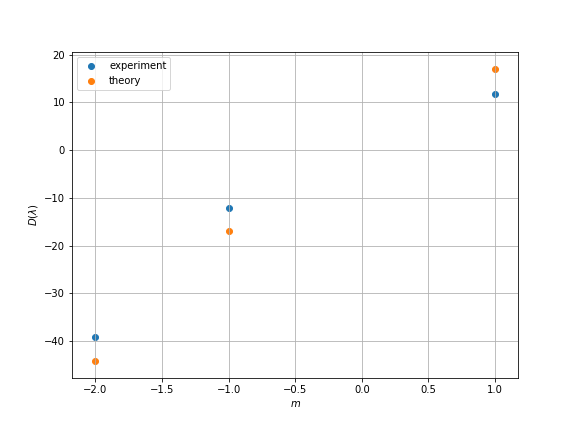
\includegraphics[width=12cm]{fig2.png}
	\caption{Угловая дисперсия.}
	\label{fig:results2}
\end{figure}

Оценим также разрешающую способность $R = \lambda / \delta \lambda$. Ширина одного желтого дуплета есть $\delta \varphi = 32^{\prime \prime}$, тогда $\delta \lambda = \delta \varphi / D \simeq 1.9 \angstrom \then R = 1.9 \cdot 10^3$. Тогда число одновременно работающих штрихов в критерии Релея $N = R/m = 1.0 \cdot 10^3$. 

\paragraph{Вывод.}
В данной работе мы научились проводить простейший спектральный анализ, а также оценили по результатам эксперимента параметры установки.

\end{document}

















